\chapter{Experimental Results}
\section {Overview}
We start by evaluating the proposed method on the data set with the least level of complexity, category 1, which contains noiseless test images given in the same orientation and scale of their corresponding models. Then we apply the method to the data set with the second lowest complexity, categories 2 and 3, and finally we evaluate the COSFIRE filters on the data set with the highest level of complexity, category 4. The mentioned order in which  the experiments are run facilitates the analysis of the performance results and gives insight on further tuning the method. The following sub-sections are the results attained for each dataset.\\

\section {Category 1 Datasets}
\subsection{Sketches25f}
This sub category of datasets is split into three different sets namely Sketches25f-level1, Sketches25f-level2, and Sketches25f-level3. Each of these data sets consist of 17 different model symbols. These model symbols consist of straight lines only and do not include any arcs or circles. This data set holds 1000 test images. This test images are given in the same orientation and in the same scale of the models. However, these test images are deformed symbols of increasing complexity according to level. Fig.\ref{fig:Sketches25fExamples} illustrates a sample of this dataset.
    
    \begin{figure*}[h]
        \centering
                \begin{subfigure}[b]{0.2\textwidth}
                \centering
                \includegraphics[width=0.73\textwidth]{figures/Results/Sketches25f/Model.png}
                \caption{Model}
        \end{subfigure}\\
                \begin{subfigure}[b]{0.25\textwidth}
                \centering
                
\includegraphics[width=0.9\textwidth]{figures/Results/Sketches25f/level1.png}
                \caption{Level 1}
        \end{subfigure}
                \begin{subfigure}[b]{0.25\textwidth}
                \centering
                \includegraphics[width=0.9\textwidth]{figures/Results/Sketches25f/level2.png}
                \caption{Level 2}
        \end{subfigure}
                \begin{subfigure}[b]{0.25\textwidth}
                \centering
                \includegraphics[width=0.9\textwidth]{figures/Results/Sketches25f/level3.png}
                \caption{Level 3}
        \end{subfigure}
        \caption[Sample data from 'Sketches25f' dataset]{Sample test images from the three different datasets under Sketches25f are shown for (a) a model symbol. (b) is a sample of Sketches25f-level1 , (c)  is a sample of Sketches25f-level2 and (d) is a sample of Sketches25f-level3.}
        \label{fig:Sketches25fExamples}
\end{figure*}

\subsubsection{Results}
\begin{table}[h]
\centering
\caption{Recognition results for dataset 'Sketches25f'}
\begin{tabular}{ccccccccccccccc}
  \hline
      Degradation Level & & & & & & & & Recognition Rate \\
  \hline
     1 & & & & & & & &  100 \% \\
     2 & & & & & & & &  100 \% \\
     3 & & & & & & & &  100 \% \\
  \hline
\end{tabular}
\end{table}



\vspace{85mm}

\subsection{Sketches25}
This sub category of datasets is split into three different sets namely Sketches25-level1, Sketches25-level2, and Sketches25-level3. Each of these data sets consist of 25 different model symbols. These model symbols consist of both straight lines and arcs or circles. This data set holds 1000 test images. This test images are given in the same orientation and in the same scale of the models. However, these test images are deformed symbols of increasing complexity according to level. Fig.\ref{fig:Sketches25Examples} illustrates a sample of this dataset.


    \begin{figure*}[h]
        \centering
                \begin{subfigure}[b]{0.2\textwidth}
                \centering
                \includegraphics[width=0.73\textwidth]{figures/Results/Sketches25/Model.png}
                \caption{Model}
        \end{subfigure}\\
                \begin{subfigure}[b]{0.25\textwidth}
                \centering
                
\includegraphics[width=0.9\textwidth]{figures/Results/Sketches25/level1.png}
                \caption{Level 1}
        \end{subfigure}
                \begin{subfigure}[b]{0.25\textwidth}
                \centering
                \includegraphics[width=0.9\textwidth]{figures/Results/Sketches25/level2.png}
                \caption{Level 2}
        \end{subfigure}
                \begin{subfigure}[b]{0.25\textwidth}
                \centering
                \includegraphics[width=0.9\textwidth]{figures/Results/Sketches25/level3.png}
                \caption{Level 3}
        \end{subfigure}
        \caption[Sample data from 'Sketches25' dataset]{Sample test images from the three different datasets under Sketches25 are shown for (a) a model symbol. (b) is a sample of Sketches25-level1 , (c)  is a sample of Sketches25-level2 and (d) is a sample of Sketches25-level3.}
        \label{fig:Sketches25Examples}
\end{figure*}

\subsubsection{Results}
\begin{table}[H]
\centering
\caption{Recognition results for dataset 'Sketches25'}
\begin{tabular}{ccccccccccccccc}
  \hline
      Degradation Level & & & & & & & & Recognition Rate \\
  \hline
     1 & & & & & & & &  100 \% \\
     2 & & & & & & & &  100 \% \\
     3 & & & & & & & &  100 \% \\
  \hline
\end{tabular}
\end{table}

\vspace{49.3mm}

\subsection{Sketches50f}
This sub category of datasets is split into three different sets namely Sketches50f-level1, Sketches50f-level2, and Sketches50f-level3. Each of these data sets consist of 26 different model symbols. These model symbols consist of straight lines only and do not include any arcs or circles. This data set holds 1000 test images. This test images are given in the same orientation and in the same scale of the models. However, these test images are deformed symbols of increasing complexity according to level. Fig.\ref{fig:Sketches50fExamples} illustrates a sample of this dataset.

    \begin{figure*}[h]
        \centering
                \begin{subfigure}[b]{0.2\textwidth}
                \centering
                \includegraphics[width=0.73\textwidth]{figures/Results/Sketches50f/Model.png}
                \caption{Model}
        \end{subfigure}\\
                \begin{subfigure}[b]{0.25\textwidth}
                \centering
                
\includegraphics[width=0.9\textwidth]{figures/Results/Sketches50f/level1.png}
                \caption{Level 1}
        \end{subfigure}
                \begin{subfigure}[b]{0.25\textwidth}
                \centering
                \includegraphics[width=0.9\textwidth]{figures/Results/Sketches50f/level2.png}
                \caption{Level 2}
        \end{subfigure}
                \begin{subfigure}[b]{0.25\textwidth}
                \centering
                \includegraphics[width=0.9\textwidth]{figures/Results/Sketches50f/level3.png}
                \caption{Level 3}
        \end{subfigure}
        \caption[Sample data from 'Sketches50f' dataset]{Sample test images from the three different datasets under Sketches50f are shown for (a) a model symbol. (b) is a sample of Sketches50f-level1 , (c)  is a sample of Sketches50f-level2 and (d) is a sample of Sketches50f-level3.}
        \label{fig:Sketches50fExamples}
\end{figure*}

\subsubsection{Results}
\begin{table}[H]
\centering
\caption{Recognition results for dataset 'Sketches50f'}
\begin{tabular}{ccccccccccccccc}
  \hline
     Degradation Level & & & & & & & & Recognition Rate \\
  \hline
     1 & & & & & & & &  100 \% \\
     2 & & & & & & & &  99.8 \% \\
     3 & & & & & & & &  99.4 \% \\

  \hline
\end{tabular}
\end{table}
\vspace{49.3mm}

\subsection{Sketches50}
This sub category of datasets is split into three different sets namely Sketches50-level1, Sketches50-level2, and Sketches50-level3. Each of these data sets consist of 50 different model symbols. These model symbols consist of both straight lines and arcs or circles. This data set holds 1000 test images. This test images are given in the same orientation and in the same scale of the models. However, these test images are deformed symbols of increasing complexity according to level. Fig.\ref{fig:Sketches50Examples} illustrates a sample of this dataset.

    \begin{figure*}[h]
        \centering
                \begin{subfigure}[b]{0.2\textwidth}
                \centering
                \includegraphics[width=0.73\textwidth]{figures/Results/Sketches50/Model.png} 
                \caption{Model}
        \end{subfigure}\\
                \begin{subfigure}[b]{0.25\textwidth}
                \centering
                
\includegraphics[width=0.9\textwidth]{figures/Results/Sketches50/level1.png}
                \caption{Level 1}
        \end{subfigure}
                \begin{subfigure}[b]{0.25\textwidth}
                \centering
                \includegraphics[width=0.9\textwidth]{figures/Results/Sketches50/level2.png}
                \caption{Level 2}
        \end{subfigure}
                \begin{subfigure}[b]{0.25\textwidth}
                \centering
                \includegraphics[width=0.9\textwidth]{figures/Results/Sketches50/level3.png}
                \caption{Level 3}
        \end{subfigure}
        \caption[Sample data from 'Sketches50' dataset]{Sample test images from the three different datasets under Sketches50 are shown for (a) a model symbol. (b) is a sample of Sketches50-level1 , (c)  is a sample of Sketches50-level2 and (d) is a sample of Sketches50-level3.}
        \label{fig:Sketches50Examples}
\end{figure*}

\subsubsection{Results}
\begin{table}[H]
\centering
\caption{Recognition results for dataset 'Sketches50'}
\begin{tabular}{ccccccccccccccc}
  \hline
     Degradation Level & & & & & & & & Recognition Rate \\
  \hline
     1 & & & & & & & &  100 \% \\
     2 & & & & & & & &  100 \% \\
     3 & & & & & & & &  100 \% \\
  \hline
\end{tabular}
\end{table}

\vspace{49.3mm}

\subsection{Sketches100f}
This sub category of datasets is split into three different sets namely Sketches100f-level1, Sketches100f-level2, and Sketches100f-level3. Each of these data sets consist of 51 different model symbols. These model symbols consist of straight lines only and do not include any arcs or circles. This data set holds 1000 test images. This test images are given in the same orientation and in the same scale of the models. However, these test images are deformed symbols of increasing complexity according to level. Fig.\ref{fig:Sketches100fExamples} illustrates a sample of this dataset.

    \begin{figure*}[h]
        \centering
                \begin{subfigure}[b]{0.2\textwidth}
                \centering
                \includegraphics[width=0.73\textwidth]{figures/Results/Sketches100f/Model.png}
                \caption{Mode}
        \end{subfigure}\\
                \begin{subfigure}[b]{0.25\textwidth}
                \centering
                
\includegraphics[width=0.9\textwidth]{figures/Results/Sketches100f/level1.png}
                \caption{level 1}
        \end{subfigure}
                \begin{subfigure}[b]{0.25\textwidth}
                \centering
                \includegraphics[width=0.9\textwidth]{figures/Results/Sketches100f/level2.png}
                \caption{level 2}
        \end{subfigure}
                \begin{subfigure}[b]{0.25\textwidth}
                \centering
                \includegraphics[width=0.9\textwidth]{figures/Results/Sketches100f/level3.png}
                \caption{level 3}
        \end{subfigure}
        \caption[Sample data from 'Sketches100f' dataset]{Sample test images from the three different datasets under Sketches100f are shown for (a) a model symbol. (b) is a sample of Sketches100f-level1 , (c)  is a sample of Sketches100f-level2 and (d) is a sample of Sketches100f-level3.}
        \label{fig:Sketches100fExamples}
\end{figure*}

\subsubsection{Results}
\begin{table}[H]
\centering
\caption{Recognition results for dataset 'Sketches100f'}
\begin{tabular}{ccccccccccccccc}
  \hline
      Degradation Level & & & & & & & & Recognition Rate \\
  \hline
     1 & & & & & & & &  98.1 \% \\
     2 & & & & & & & &  98.7 \% \\
     3 & & & & & & & &  98.1 \% \\

  \hline
\end{tabular}
\end{table}

\vspace{49.3mm}

\subsection{Sketches100}
This sub category of datasets is split into three different sets namely Sketches100-level1, Sketches100-level2, and Sketches500-level3. Each of these data sets consist of 100 different model symbols. These model symbols consist of both straight lines and arcs or circles. This data set holds 1000 test images. This test images are given in the same orientation and in the same scale of the models. However, these test images are deformed symbols of increasing complexity according to level. Fig.\ref{fig:Sketches100Examples} illustrates a sample of this dataset.

    \begin{figure*}[h]
        \centering
                \begin{subfigure}[b]{0.2\textwidth}
                \centering
                \includegraphics[width=0.73\textwidth]{figures/Results/Sketches100/Models.png}
                \caption{Model}
                \end{subfigure}\\
                \begin{subfigure}[b]{0.25\textwidth}
                \centering
                
\includegraphics[width=0.9\textwidth]{figures/Results/Sketches100/level1.png}
                \caption{Level 1}
        \end{subfigure}
                \begin{subfigure}[b]{0.25\textwidth}
                \centering
                \includegraphics[width=0.9\textwidth]{figures/Results/Sketches100/level2.png}
                \caption{Level 2}
        \end{subfigure}
                \begin{subfigure}[b]{0.25\textwidth}
                \centering
                \includegraphics[width=0.9\textwidth]{figures/Results/Sketches100/level3.png}
                \caption{Level 3}
        \end{subfigure}
        \caption[Sample data from 'Sketches100' dataset]{Sample test images from the three different datasets under Sketches100 are shown for (a) a model symbol. (b) is a sample of Sketches100-level1 , (c)  is a sample of Sketches100-level2 and (d) is a sample of Sketches100-level3.}
        \label{fig:Sketches100Examples}
\end{figure*}

\subsubsection{Results}
\begin{table}[H]
\centering
\caption{Recognition results for dataset 'Sketches100'}
\begin{tabular}{ccccccccccccccc}
  \hline
     Degradation Level & & & & & & & & Recognition Rate \\
  \hline
     1 & & & & & & & &  99.2 \% \\
     2 & & & & & & & &  98.9 \% \\
     3 & & & & & & & &  98.2 \% \\

  \hline
\end{tabular}
\end{table}

\vspace{49.3mm}

\subsection{Sketches150f}
This sub category of datasets is split into three different sets namely Sketches150f-level1, Sketches150f-level2, and Sketches150f-level3. Each of these data sets consist of 80 different model symbols. These model symbols consist of straight lines only and do not include any arcs or circles. This data set holds 1000 test images. This test images are given in the same orientation and in the same scale of the models. However, these test images are deformed symbols of increasing complexity according to level. Fig.\ref{fig:Sketches150fExamples} illustrates a sample of this dataset.

    \begin{figure*}[h]
        \centering
                \begin{subfigure}[b]{0.2\textwidth}
                \centering
                \includegraphics[width=0.73\textwidth]{figures/Results/Sketches150f/Model.png}
                \caption{Model}
        \end{subfigure}\\
                \begin{subfigure}[b]{0.25\textwidth}
                \centering
                
\includegraphics[width=0.9\textwidth]{figures/Results/Sketches150f/level1.png}
                \caption{Level 1}
        \end{subfigure}
                \begin{subfigure}[b]{0.25\textwidth}
                \centering
                \includegraphics[width=0.9\textwidth]{figures/Results/Sketches150f/level2.png}
                \caption{Level 2}
        \end{subfigure}
                \begin{subfigure}[b]{0.25\textwidth}
                \centering
                \includegraphics[width=0.9\textwidth]{figures/Results/Sketches150f/level3.png}
                \caption{Level 3}
        \end{subfigure}
        \caption[Sample data from 'Sketches150f' dataset]{Sample test images from the three different datasets under Sketches150f are shown for (a) a model symbol. (b) is a sample of Sketches150f-level1 , (c)  is a sample of Sketches150f-level2 and (d) is a sample of Sketches150f-level3.}
        \label{fig:Sketches150fExamples}
\end{figure*}


\subsubsection{Results}
\begin{table}[H]
\centering
\caption{Recognition results for dataset 'Sketches150f'}
\begin{tabular}{ccccccccccccccc}
  \hline
      Degradation Level & & & & & & & & Recognition Rate \\
  \hline
     1 & & & & & & & &  99.3 \% \\
     2 & & & & & & & &  99.2 \% \\
     3 & & & & & & & &  98.8 \% \\

  \hline
\end{tabular}
\end{table}
\vspace{49.3mm}

\subsection{Sketches150}
This sub category of datasets is split into three different sets namely Sketches150-level1, Sketches150-level2, and Sketches150-level3. Each of these data sets consist of 150 different model symbols. These model symbols consist of both straight lines and arcs or circles. This data set holds 1000 test images. These test images are given in the same orientation and in the same scale of the models. However, these test images are deformed symbols of increasing complexity according to level. Fig.\ref{fig:Sketches150Examples} illustrates a sample of this dataset.

    \begin{figure*}[h]
        \centering
                \begin{subfigure}[b]{0.2\textwidth}
                \centering
                \includegraphics[width=0.73\textwidth]{figures/Results/Sketches150/Model.png}
                \caption{Model}
        \end{subfigure}\\
                \begin{subfigure}[b]{0.25\textwidth}
                \centering
                
\includegraphics[width=0.9\textwidth]{figures/Results/Sketches150/level1.png}
                \caption{Level 1}
        \end{subfigure}
                \begin{subfigure}[b]{0.25\textwidth}
                \centering
                \includegraphics[width=0.9\textwidth]{figures/Results/Sketches150/level2.png}
                \caption{Level 2}
        \end{subfigure}
                \begin{subfigure}[b]{0.25\textwidth}
                \centering
                \includegraphics[width=0.9\textwidth]{figures/Results/Sketches150/level3.png}
                \caption{Level 3}
        \end{subfigure}
        \caption[Sample data from 'Sketches150' dataset]{Sample test images from the three different datasets under Sketches150 are shown for (a) a model symbol. (b) is a sample of Sketches150-level1 , (c)  is a sample of Sketches150-level2 and (d) is a sample of Sketches150-level3.}
        \label{fig:Sketches150Examples}
\end{figure*}

\subsubsection{Results}
\begin{table}[H]
\centering
\caption{Recognition results for dataset 'Sketches150'}
\begin{tabular}{ccccccccccccccc}
  \hline
      Degradation Level & & & & & & & & Recognition Rate \\
  \hline
     1 & & & & & & & &  99.3 \% \\
     2 & & & & & & & &  98.9 \% \\
     3 & & & & & & & &  97.6 \% \\

  \hline
\end{tabular}
\end{table}
\vspace{49.3mm}


\section {Category 2 Datasets}
\subsection{Rotation}
This data set consists of 150 different models and 10 test symbols for each of those models.These model symbols consist of both straight lines and arcs or circles. In total this dataset holds 1500 test images. The test images are given in the same scale of the models. Orientation varies through out the 25 test symbols for each model. No noise is introduced to the test images. Fig. \ref{fig:RotationExamples} illustrates a few samples.

    \begin{figure*}[h]
    
        \centering
                \begin{subfigure}[b]{0.2\textwidth}
                \centering
                \includegraphics[width=0.81\textwidth]{figures/Results/Rotation/Model.png}
                \caption{}
        \end{subfigure}\\
                \begin{subfigure}[b]{0.25\textwidth}
                \centering
                \includegraphics[width=0.85\textwidth]{figures/Results/Rotation/1.png}
                \put(8,40){$\cdots$}
                \caption{}
        \end{subfigure}
        \qquad
                \begin{subfigure}[b]{0.25\textwidth}
                \centering
                \includegraphics[width=0.9\textwidth]{figures/Results/Rotation/2.png}
                \put(8,40){$\cdots$}
                \caption{}
        \end{subfigure}
        \qquad
                \begin{subfigure}[b]{0.25\textwidth}
                \centering
                \includegraphics[width=0.7\textwidth]{figures/Results/Rotation/3.png}
                \caption{}
        \end{subfigure}
        \caption[Sample data from the 'Rotation' dataset]{(b) (c) (d) Three test images for (a) a model symbol are illustrated from the Rotation dataset }
        \label{fig:RotationExamples}
\end{figure*}

\subsubsection{Results}
\begin{table}[H]
\centering
\caption{Recognition results for dataset 'Rotation'}
\begin{tabular}{ccccccccccccccc}
  \hline
      Recognition Rate \\
  \hline
      72.6 \% \\
  \hline
\end{tabular}
\end{table}
\vspace{85mm}

\subsection{Scaling}
This data set consists of 150 different models and 10 test symbols for each of those models.These model symbols consist of both straight lines and arcs or circles. In total this dataset holds 1500 test images. The test images are given in the same orientation of the models. Scaling varies through out the 25 test symbols for each model. No noise is introduced to the test images. Fig. \ref{fig:ScalingExamples} illustrates a few samples.

    \begin{figure*}[h]
        \centering
                \begin{subfigure}[b]{0.2\textwidth}
                \centering
                \includegraphics[width=0.73\textwidth]{figures/Results/Scaling/Model.png}
                \caption{}
        \end{subfigure}\\
                \begin{subfigure}[b]{0.25\textwidth}
                \centering
                \includegraphics[width=0.9\textwidth]{figures/Results/Scaling/1.png}
                \put(8,40){$\cdots$}
                \caption{}
        \end{subfigure}
        \qquad
                \begin{subfigure}[b]{0.25\textwidth}
                \centering
                \includegraphics[width=0.9\textwidth]{figures/Results/Scaling/2.png}
                \put(8,40){$\cdots$}
                \caption{}
        \end{subfigure}
        \qquad
                \begin{subfigure}[b]{0.25\textwidth}
                \centering
                \includegraphics[width=0.9\textwidth]{figures/Results/Scaling/3.png}
                \caption{}
        \end{subfigure}
        \caption[Sample data from the 'Scaling' dataset]{(b) (c) (d) Three test images for (a) a model symbol are illustrated from the Scaling dataset }
        \label{fig:ScalingExamples}
\end{figure*}

\subsubsection{Results}
\begin{table}[H]
\centering
\caption{Recognition results for dataset 'Scaling'}
\begin{tabular}{ccccccccccccccc}
  \hline
      Recognition Rate \\
  \hline
      89.5 \% \\
  \hline
\end{tabular}
\end{table}
\vspace{85mm}

\subsection{RotationScaling}    
This data set consists of 150 different models and 10 test symbols for each of those models.These model symbols consist of both straight lines and arcs or circles. In total this dataset holds 1500 test images. Scaling and orientation vary from those in the model through out each of the 25 test symbols. No noise is introduced to the test images. Fig. \ref{fig:RotationScalingExamples} illustrates a few samples.

\begin{figure*}[h]
        \centering
                \begin{subfigure}[b]{0.2\textwidth}
                \centering
                \includegraphics[width=0.73\textwidth]{figures/Results/RotationScaling/Model.png}
                \caption{}
        \end{subfigure}\\
                \begin{subfigure}[b]{0.25\textwidth}
                \centering
                \includegraphics[width=0.9\textwidth]{figures/Results/RotationScaling/1.png}
                \put(8,40){$\cdots$}
                \caption{}
        \end{subfigure}
        \qquad
                \begin{subfigure}[b]{0.25\textwidth}
                \centering
                \includegraphics[width=0.9\textwidth]{figures/Results/RotationScaling/2.png}
                \put(8,40){$\cdots$}
                \caption{}
        \end{subfigure}
        \qquad
                \begin{subfigure}[b]{0.25\textwidth}
                \centering
                \includegraphics[width=0.9\textwidth]{figures/Results/RotationScaling/3.png}
                \caption{}
        \end{subfigure}
        \caption[Sample data from the 'RotationScaling' dataset]{(b) (c) (d) Three test images for (a) a model symbol are illustrated from the RotationScaling dataset }
        \label{fig:RotationScalingExamples} 
\end{figure*}        

\subsubsection{Results}
\begin{table}[H]
\centering
\caption{Recognition results for dataset 'RotationScaling'}
\begin{tabular}{ccccccccccccccc}
  \hline
      Recognition Rate \\
  \hline
      49.2 \% \\
  \hline
\end{tabular}
\end{table}
\vspace{85mm}


\section {Category 3 Datasets}
\subsection{Noise A}
This data set consists of 150 different models and 25 test symbols for each of those models.These model symbols consist of both straight lines and arcs or circles. In total this dataset holds 3750 test images. The test images are given in the same orientation and in the same scale of the models. Noise is introduced to the test images in the form of line degradation. Fig. \ref{fig:NoiseAExamples} illustrates a few samples.

    \begin{figure*}[h]
        \centering
                \begin{subfigure}[b]{0.2\textwidth}
                \centering
                \includegraphics[width=1.1\textwidth]{figures/Results/NoiseA/Model.png}
                \caption{}
        \end{subfigure}\\
                \begin{subfigure}[b]{0.25\textwidth}
                \centering
                \includegraphics[width=0.9\textwidth]{figures/Results/NoiseA/1.png}
                \put(8,40){$\cdots$}
                \caption{}
        \end{subfigure}
        \qquad
                \begin{subfigure}[b]{0.25\textwidth}
                \centering
                \includegraphics[width=0.9\textwidth]{figures/Results/NoiseA/2.png}
                \put(8,40){$\cdots$}
                \caption{}
        \end{subfigure}
        \qquad
                \begin{subfigure}[b]{0.25\textwidth}
                \centering
                \includegraphics[width=0.9\textwidth]{figures/Results/NoiseA/3.png}
                \caption{}
        \end{subfigure}
        \caption[Sample data from the 'Noise A' dataset]{(b) (c) (d) Three test images for (a) a model symbol are illustrated from the Noise A }
        \label{fig:NoiseAExamples}
\end{figure*}

\subsubsection{Results}
\begin{table}[H]
\centering
\caption{Recognition results for dataset 'Noise A'}
\begin{tabular}{ccccccccccccccc}
  \hline
      Recognition Rate \\
  \hline
      96.13 \% \\
  \hline
\end{tabular}
\end{table}
\vspace{49.3mm}

\subsection{Noise B}
This data set consists of 150 different models and 25 test symbols for each of those models.These model symbols consist of both straight lines and arcs or circles. In total this dataset holds 3750 test images. The test images are given in the same orientation and in the same scale of the models. Noise is introduced to the test images in the form of line thickening. Fig. \ref{fig:NoiseBExamples} illustrates a few samples.

    \begin{figure*}[h]
        \centering
                \begin{subfigure}[b]{0.2\textwidth}
                \centering
                \includegraphics[width=1.1\textwidth]{figures/Results/NoiseB/Model.png}
                \caption{}
        \end{subfigure}\\
                \begin{subfigure}[b]{0.25\textwidth}
                \centering
                \includegraphics[width=0.9\textwidth]{figures/Results/NoiseB/1.png}
                \put(8,40){$\cdots$}
                \caption{}
        \end{subfigure}
        \qquad
                \begin{subfigure}[b]{0.25\textwidth}
                \centering
                \includegraphics[width=0.9\textwidth]{figures/Results/NoiseB/2.png}
                \put(8,40){$\cdots$}
                \caption{}
        \end{subfigure}
        \qquad
                \begin{subfigure}[b]{0.25\textwidth}
                \centering
                \includegraphics[width=0.9\textwidth]{figures/Results/NoiseB/3.png}
                \caption{}
        \end{subfigure}
        \caption[Sample data from the 'Noise B' dataset]{(b) (c) (d) Three test images for (a) a model symbol are illustrated from the Noise B }
        \label{fig:NoiseBExamples}
\end{figure*}

\subsubsection{Results}
\begin{table}[H]
\centering
\caption{Recognition results for dataset 'Noise B'}
\begin{tabular}{ccccccccccccccc}
  \hline
      Recognition Rate \\
  \hline
      90.8 \% \\
  \hline
\end{tabular}
\end{table}
\vspace{65mm}

\subsection{Noise E}    
This data set consists of 150 different models and 25 test symbols for each of those models. These model symbols consist of both straight lines and arcs or circles. In total this dataset holds 3750 test images. The test images are given in the same orientation and in the same scale of the models. Noise is introduced to the test images in the form of of global noise. Fig. \ref{fig:NoiseEExamples} illustrates a few samples.
    
    \begin{figure*}[h]
        \centering
                \begin{subfigure}[b]{0.2\textwidth}
                \centering
                \includegraphics[width=1.1\textwidth]{figures/Results/NoiseE/Model.png}
                \caption{}
        \end{subfigure}\\
                \begin{subfigure}[b]{0.25\textwidth}
                \centering
                \includegraphics[width=0.9\textwidth]{figures/Results/NoiseE/1.png}
                \put(8,40){$\cdots$}
                \caption{}
        \end{subfigure}
        \qquad
                \begin{subfigure}[b]{0.25\textwidth}
                \centering
                \includegraphics[width=0.9\textwidth]{figures/Results/NoiseE/2.png}
                \put(8,40){$\cdots$}
                \caption{}
        \end{subfigure}
        \qquad
                \begin{subfigure}[b]{0.25\textwidth}
                \centering
                \includegraphics[width=0.9\textwidth]{figures/Results/NoiseE/3.png}
                \caption{}
        \end{subfigure}
        \caption[Sample data from the 'Noise E' dataset]{(b) (c) (d) Three test images for (a) a model symbol are illustrated from the Noise E dataset }
        \label{fig:NoiseEExamples}
\end{figure*}

\subsubsection{Results}
\begin{table}[H]
\centering
\caption{Recognition results for dataset 'Noise E'}
\begin{tabular}{ccccccccccccccc}
  \hline
      Recognition Rate \\
  \hline
      94.93 \% \\
  \hline
\end{tabular}
\end{table}
\vspace{65mm}